\chapter{Shallow Neural Networks}
\section{Activation Functions}

\subsection{Rectified Linear Unit (ReLU)}

The ReLU activation function is defined as:

\begin{figure}[ht]
\centering
\begin{minipage}{0.4\textwidth}
\begin{tikzpicture}[domain=-3:3, scale=1]
    % Draw axes
    \draw[->] (-3.5,0) -- (3.5,0) node[right] {$z$};
    \draw[->] (0,-0.5) -- (0,3.5) node[above] {$ReLu(z)$};
    
    % Draw ReLU function: y = 0 for x < 0
    \draw[blue, thick] plot[domain=-3:0] (\x, 0);
    
    % Draw ReLU function: y = x for x >= 0
    \draw[blue, thick] plot[domain=0:3] (\x, {\x});
\end{tikzpicture}
\end{minipage}%
\begin{minipage}{0.4\textwidth}
$
\color{blue}{
f(x) = \max(0, x) = 
\begin{cases}
0, & \text{if } x < 0 \\
x, & \text{if } x \geq 0
\end{cases}
}
$
\end{minipage}
\caption{Rectified Linear Unit (ReLU) activation function}
\label{fig:relu}
\end{figure}

\subsection{Elements of the family F}

$$
y = \phi_0 + \phi_1 a[\theta_{10} + \theta_{11} x] + \phi_2 a[\theta_{20} + \theta_{21} x] + \phi_3 a[\theta_{30} + \theta_{31} x]
$$

\begin{figure}[H]
    \centering
    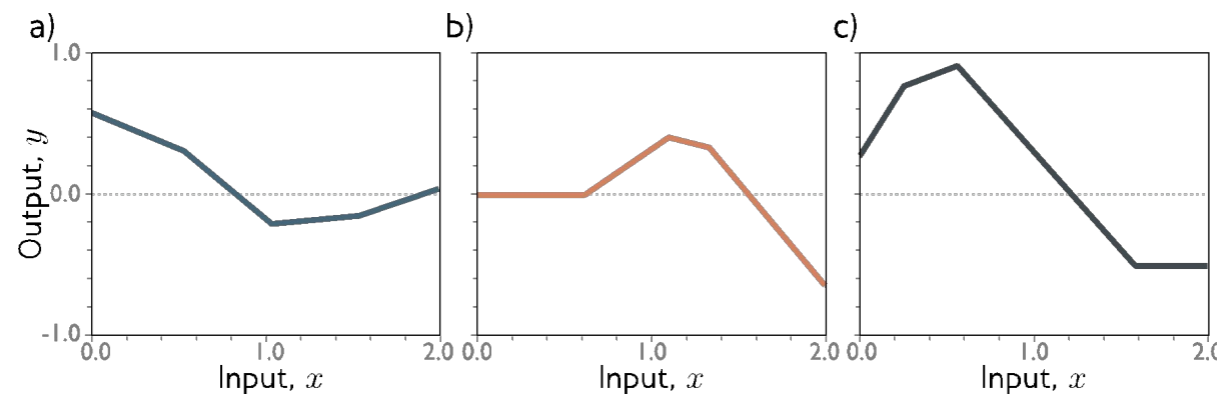
\includegraphics[width=0.7\textwidth]{assets/abc_foo.png}
    \caption{Family of functions $F$}
    \label{fig:family_f}
\end{figure}

$$
\begin{cases}
    z_1 = \phi(a_1) = \phi_0 + \phi_1 a[\theta_{10} + \theta_{11} x]
    \\
    z_2 = \phi(a_2) = \phi_0 + \phi_2 a[\theta_{20} + \theta_{21} x]
    \\
    z_3 = \phi(a_3) = \phi_0 + \phi_3 a[\theta_{30} + \theta_{31} x]
\end{cases}
$$

\begin{center}
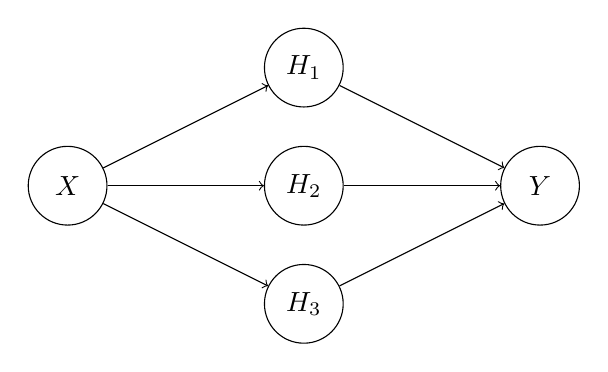
\begin{tikzpicture}[x=2cm, y=1.5cm, every node/.style={circle, draw, minimum size=1cm}]
    % Input layer (3 neurons)
    \node[] (X) at (0,-2) {$X$};
    
    % Hidden layer (3 neurons)
    \foreach \j in {1,...,3} {
        \node[] (H\j) at (1.5,-\j) {$H_{\j}$};
    }
    
    % Output layer (1 neuron)
    \node[] (Y) at (3,-2) {$Y$};
    
    % Connect input layer to hidden layer
    \foreach \j in {1,...,3} {
        \draw[->] (X) -- (H\j);
    }
    
    % Connect hidden layer to output layer
    \foreach \j in {1,...,3} {
        \draw[->] (H\j) -- (Y);
    }
\end{tikzpicture}
\end{center}


$$
y = W^{(2)} \phi (W^{(1)} x + b^{(1)}) + b^{(2)}
$$

$$
W^* = W^{(2)} W^{(1)} \quad \quad \text{rank}(W^*) = \min
$$

\dots

\begin{figure}[H]
    \centering
    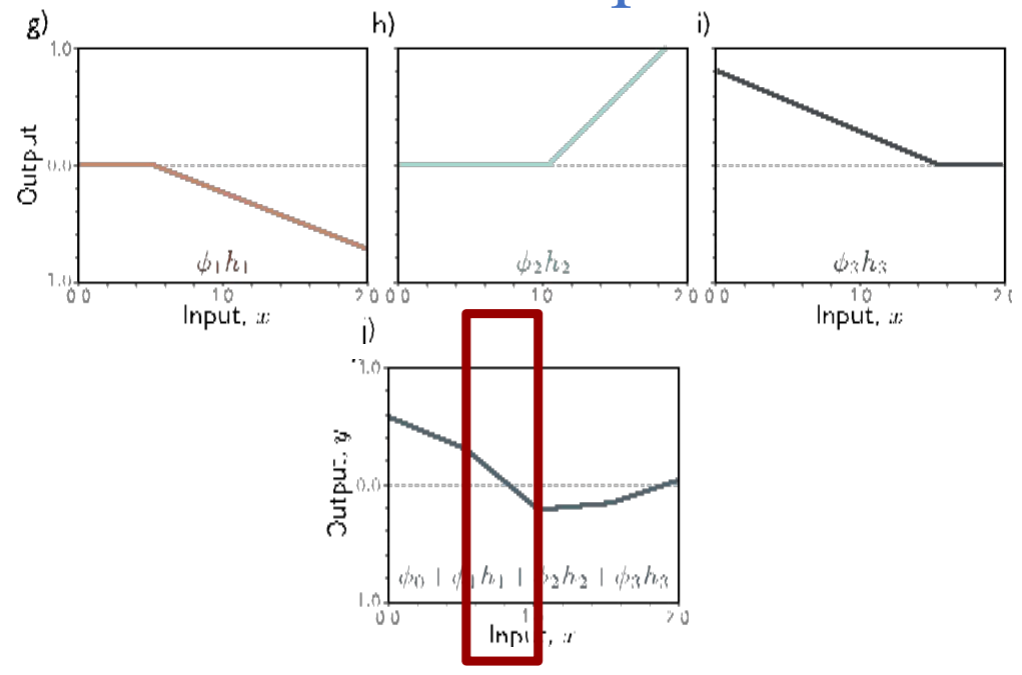
\includegraphics[width=0.7\textwidth]{assets/flow_comp.png}
    \caption{Flow computation}
    \label{fig:flow_comp}
\end{figure}

In the hilighted section, the contribute of the 2nd neuron of the hidden layer is zero, so the output is only influenced by the 1st and 3rd neurons of the hidden layer.

This is a consequence of the ReLU activation function, which deactivates the second node in that interval of the input space:

\begin{center}
    \usetikzlibrary{shapes.misc}
    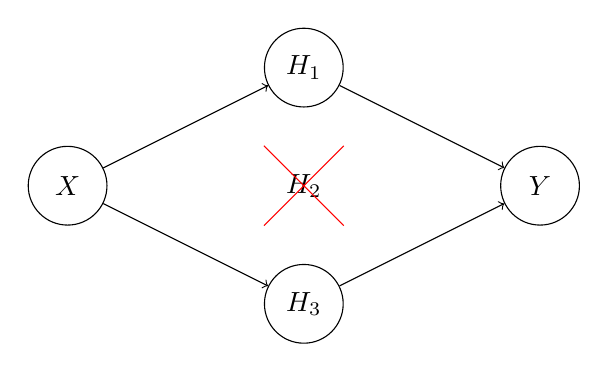
\begin{tikzpicture}[x=2cm, y=1.5cm, every node/.style={circle, draw, minimum size=1cm}]
        % Input layer (3 neurons)
        \node[] (X) at (0,-2) {$X$};
        
        % Hidden layer (3 neurons)
        \node[] (H1) at (1.5,-1) {$H_{1}$};
        \node[circle, draw=black, cross out, draw=red] (H2) at (1.5,-2) {$H_{2}$};
        \node[] (H3) at (1.5,-3) {$H_{3}$};
        
        % Output layer (1 neuron)
        \node[] (Y) at (3,-2) {$Y$};
        
        % Connect input layer to hidden layer
        \foreach \j in {1, 3} {
            \draw[->] (X) -- (H\j);
        }
        
        % Connect hidden layer to output layer
        \foreach \j in {1, 3} {
            \draw[->] (H\j) -- (Y);
        }
    \end{tikzpicture}
\end{center}


\subsubsection{Multivariate Output}

For multivariate output, the situation is similar to the previous case. In this case, the output layer has two neurons, $Y_1$ and $Y_2$:

\begin{center}
    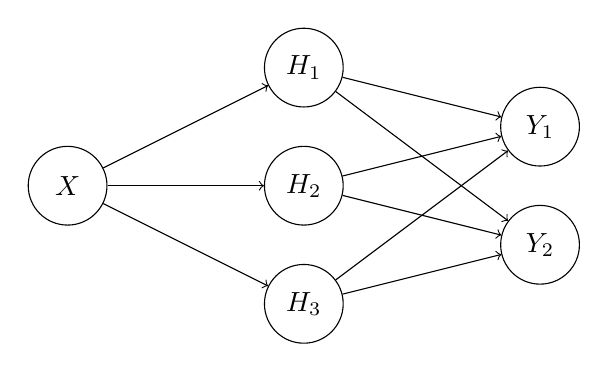
\begin{tikzpicture}[x=2cm, y=1.5cm, every node/.style={circle, draw, minimum size=1cm}]
        % Input layer (3 neurons)
        \node[] (X) at (0,-2) {$X$};
        
        % Hidden layer (3 neurons)
        \foreach \j in {1,...,3} {
            \node[] (H\j) at (1.5,-\j) {$H_{\j}$};
        }
        
        % Output layer (1 neuron)
        \node[] (Y1) at (3,-1.5) {$Y_1$};
        \node[] (Y2) at (3,-2.5) {$Y_2$};
        
        % Connect input layer to hidden layer
        \foreach \j in {1,...,3} {
            \draw[->] (X) -- (H\j);
        }
        
        % Connect hidden layer to output layer
        \foreach \i in {1, 2} {
            \foreach \j in {1,...,3} {
                \draw[->] (H\j) -- (Y\i);
            }
        }
    \end{tikzpicture}
\end{center}

We obtain the output as:

\begin{figure}[H]
    \centering
    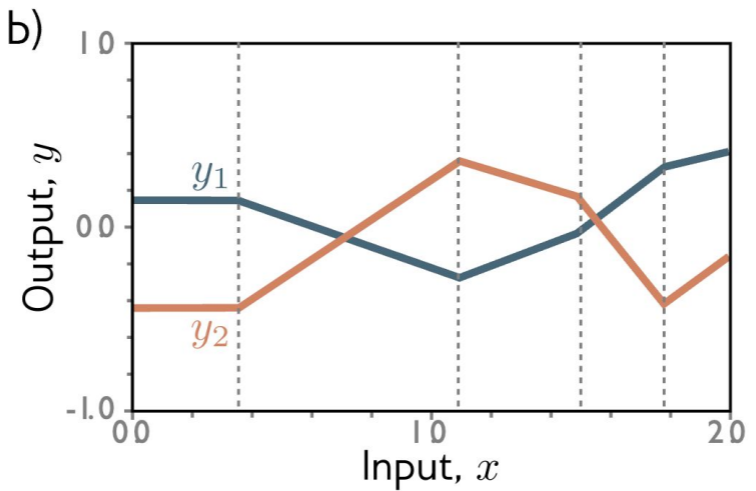
\includegraphics[width=0.5\textwidth]{assets/mult_out.png}
    \caption{Flow computation for multivariate output}
    \label{fig:multi_out}
\end{figure}

\subsubsection{Multivariate Input}

\tikzset{
  functions/.style={draw, minimum width=3cm, minimum height=3cm}
}

\begin{center}
    
    \begin{minipage}{0.4\textwidth}
        \begin{center}
            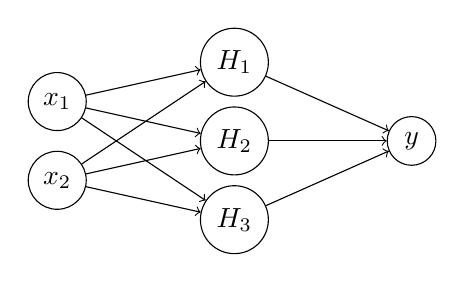
\begin{tikzpicture}[x=1.5cm, y=1cm, every node/.style={circle, draw, minimum size=0.5cm}]
                % Input layer (2 neurons)
                \node[] (X1) at (0,-1.5) {$x_1$};
                \node[] (X2) at (0,-2.5) {$x_2$};
                
                % Hidden layer (3 neurons)
                \foreach \j in {1,...,3} {
                    \node[] (H\j) at (1.5,-\j) {$H_{\j}$};
                }
                
                % Output layer (1 neuron)
                \node[] (Y) at (3,-2) {$y$};
                
                % Connect input layer to hidden layer
                \foreach \i in {1,2} {
                    \foreach \j in {1,...,3} {
                        \draw[->] (X\i) -- (H\j);
                    }
                }
                
                % Connect hidden layer to output layer
                \foreach \j in {1,...,3} {
                    \draw[->] (H\j) -- (Y);
                }
            \end{tikzpicture}
        \end{center}
    \end{minipage}
    \begin{minipage}{0.55\textwidth}
        \begin{figure}[H]
            \centering
            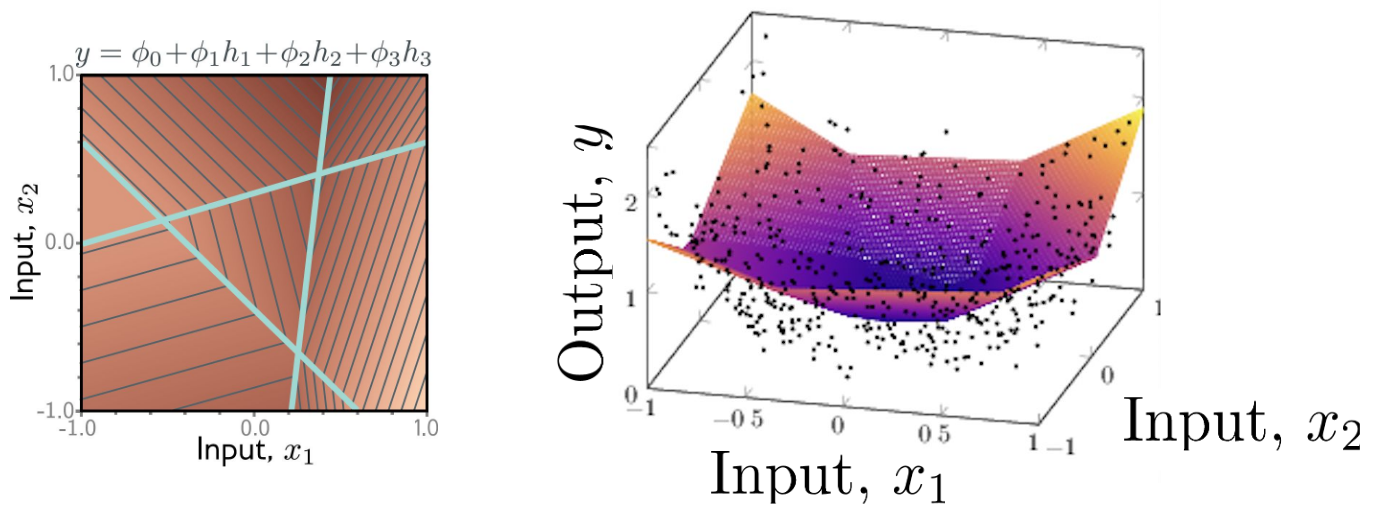
\includegraphics[width=\textwidth]{assets/multi_input_out.png}
            \label{fig:multi_in}
        \end{figure}
    \end{minipage}
\end{center}
                    
In this case we have 13 parameters:

\begin{itemize}
    \item We have 3 parameters from $X_1$ and $X_2$ to connect each node of the hidden layer (2 are the weights and 1 is the bias), for a total of 9 parameters.
    \item We have 4 parameters from the hidden layer to the output layer (3 weights and the bias term).
\end{itemize}

The general formula to count the number of parameters is:

$$
\#
$$

\begin{center}
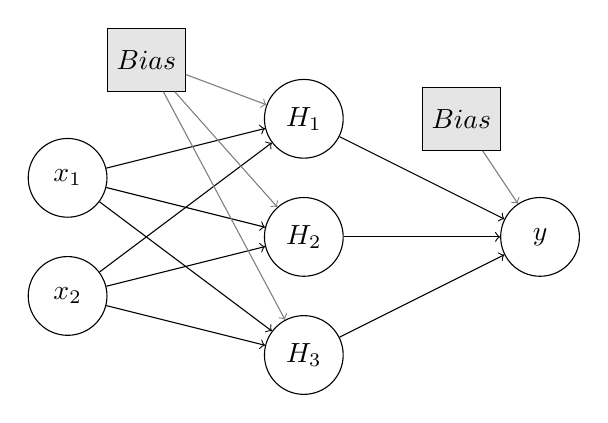
\begin{tikzpicture}[x=2cm, y=1.5cm, every node/.style={circle, draw, minimum size=1cm}]
    % Input layer (2 neurons)
    \node[] (X1) at (0,-1.5) {$x_1$};
    \node[] (X2) at (0,-2.5) {$x_2$};
    % Bias for hidden layer (displayed as a rectangle)
    \node[rectangle, draw, fill=gray!20, minimum size=0.8cm] (B1) at (0.5,-0.5) {$Bias$};
    
    % Hidden layer (3 neurons)
    \foreach \j in {1,...,3} {
        \node[] (H\j) at (1.5,-\j) {$H_{\j}$};
    }
    % Bias for output layer (displayed as a rectangle)
    \node[rectangle, draw, fill=gray!20, minimum size=0.8cm] (B2) at (2.5,-1) {$Bias$};
    
    % Output layer (1 neuron)
    \node[] (Y) at (3,-2) {$y$};
    
    % Connections: Input to Hidden
    \foreach \i in {1,2} {
        \foreach \j in {1,...,3} {
            \draw[->] (X\i) -- (H\j);
        }
    }
    % Bias B1 to all hidden neurons
    \foreach \j in {1,...,3} {
         \draw[->, gray] (B1) -- (H\j);
    }
    
    % Connections: Hidden to Output
    \foreach \j in {1,...,3} {
        \draw[->] (H\j) -- (Y);
    }
    % Bias B2 to output neuron
    \draw[->, gray] (B2) -- (Y);
\end{tikzpicture}
\end{center}

\subsubsection{General Case}


\begin{center}
    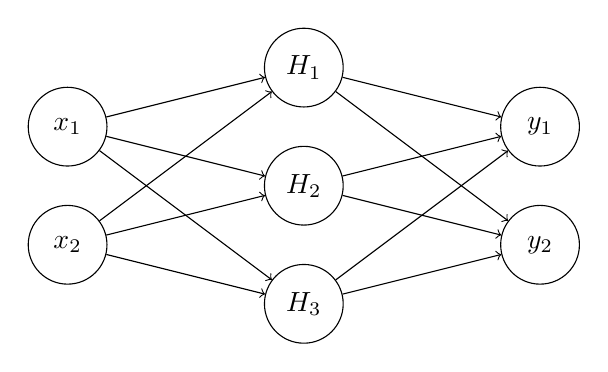
\begin{tikzpicture}[x=2cm, y=1.5cm, every node/.style={circle, draw, minimum size=1cm}]
        % Input layer (2 neurons)
        \node[] (X1) at (0,-1.5) {$x_1$};
        \node[] (X2) at (0,-2.5) {$x_2$};
        
        % Hidden layer (3 neurons)
        \foreach \j in {1,...,3} {
            \node[] (H\j) at (1.5,-\j) {$H_{\j}$};
        }
        
        % Output layer (2 neuron)
        \node[] (Y1) at (3,-1.5) {$y_1$};
        \node[] (Y2) at (3,-2.5) {$y_2$};
        
        % Connect input layer to hidden layer
        \foreach \i in {1,2} {
            \foreach \j in {1,...,3} {
                \draw[->] (X\i) -- (H\j);
            }
        }
        
        % Connect hidden layer to output layer
        \foreach \i in {1, 2} {
            \foreach \j in {1,...,3} {
                \draw[->] (H\j) -- (Y\i);
            }
        }
    \end{tikzpicture}
\end{center}

% \subsubsection{Batches}

% We can divide data in $M$ batches of $B$ data points each, such that $M\cdot B = N$:

% $$
% \left.
% \begin{array}{|c|}
%     \hline
%     B\\
%     \hline
%     B\\
%     \hline
%     \vdots\\
%     \hline
%     B\\
%     \hline
% \end{array}
% \right\} M
% $$